% Author: Izaak Neutelings (February 2019)
\documentclass[border=3pt,tikz]{standalone}
\usepackage{physics}
\usepackage{tikz}
\usetikzlibrary{patterns,decorations.pathmorphing}
\usetikzlibrary{arrows.meta}
\tikzset{>=latex}

\colorlet{mydarkblue}{blue!50!black}
\colorlet{myblue}{blue!30}
\colorlet{mydarkred}{red!60!black}
\colorlet{myred}{red!30}
\colorlet{mydarkgreen}{green!60!black}
\colorlet{mygreen}{green!30}
\colorlet{mydarkorange}{yellow!40!red}
\colorlet{myorange}{yellow!80!red}
\colorlet{myyellow}{yellow!80}
\colorlet{mygrey}{black!15}
\colorlet{mydarkgrey}{black!50}

\tikzstyle{piston}=[blue!50!black,top color=blue!30,bottom color=blue!50,middle color=blue!20,shading angle=0]
\tikzstyle{walldark}=[blue!20!black,top color=black!10!white!90!blue,bottom color=black!20!white!90!blue,shading angle=-30]
\tikzstyle{wall}=[blue!20!black,top color=black!5!white!90!blue,bottom color=black!10!white!85!blue,shading angle=30]

% GAS MOLECULE with vector
\tikzset{
  gasparticle/.pic={
    \tikzset{/gasparticle/.cd,#1}
    \draw[-{Latex[length=4,width=3]},green!60!black,thick] (0,0) -- (\vec);
    \node[circle,fill,inner sep=1.5,fill=black!80!blue] at (0,0) {};
  }
  /gasparticle/.search also={/tikz},
  /gasparticle/.cd,
  vec/.store in=\vec, vec={90:0.5},
}

\begin{document}

% PISTON
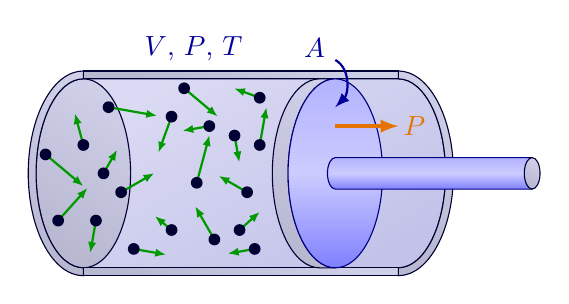
\begin{tikzpicture}
  \def\Ra{0.6}
  \def\Rb{1.2}
  \def\ra{0.1}
  \def\rb{0.2}
  \def\w{0.10} % wall thickness
  \def\x{3.2}  % piston position
  \def\L{4}    % container length
  \def\l{2.5}  % piston length
  \def\v{0.7}  % piston length
  
  % WALL
  \draw[wall]
    (0,\Rb) -- (0,-\Rb) --++ (\L,0) arc (-90:90:{\Ra} and {\Rb}) -- cycle;
  \draw[walldark] (0,0) ellipse ({\Ra} and \Rb);
  
  % SHELL
  \draw[walldark]
    (0,\Rb) rectangle++ (\L,\w);
  \draw[walldark]
    (0,-\Rb) rectangle++ (\L,-\w);
  \draw[walldark]
    (\L,\Rb+\w) arc (90:-90:{\Ra+\w} and {\Rb+\w}) --++ (0,\w) arc (-90:90:{\Ra} and {\Rb}) -- cycle;
  \draw[walldark]
    (0,\Rb) arc (90:270:{\Ra} and {\Rb}) --++ (0,-\w) arc (-90:-270:{\Ra+\w} and {\Rb+\w}) -- cycle;
  
  % PISTON
  \draw[walldark]
    (\x,\Rb) arc (90:270:{\Ra} and {\Rb}) --++ (-2*\w,0) arc (-90:-270:{\Ra} and {\Rb}) -- cycle;
  \draw[piston] (\x,0) ellipse ({\Ra} and \Rb);
  \draw[piston]
    (\x,\rb) arc (90:270:{\ra} and {\rb}) --++ (\l,0) --++ (0,2*\rb) -- cycle;
  \draw[walldark] (\x+\l,0) ellipse ({\ra} and \rb);
  
  % LABELS
  \draw[->,very thick,orange!90!black] (\x,0.5*\Rb) --++ (0.2*\L,0)
    node[right=-2,orange!90!black] {$P$};
  \node[right,blue!60!black,above] at (\L/2-\Ra,\Rb+\w) {$V$, $P$, $T$};
  \draw[<-,thick,blue!60!black] (\x,0.7*\Rb) to[in=-30] (\x,1.2*\Rb)
    node[below=3,above left] {$A$};
  
  % GAS PARTICLE
  \pic at (-0.15*\x, 0.2*\Rb) {gasparticle={vec={ -40:0.9*\v}}};
  \pic at (-0.10*\x,-0.5*\Rb) {gasparticle={vec={  48:0.8*\v}}};
  \pic at ( 0.00*\x, 0.3*\Rb) {gasparticle={vec={ 105:0.6*\v}}};
  \pic at ( 0.05*\x,-0.5*\Rb) {gasparticle={vec={-100:0.6*\v}}};
  \pic at ( 0.08*\x, 0.0*\Rb) {gasparticle={vec={  60:0.5*\v}}};
  \pic at ( 0.10*\x, 0.7*\Rb) {gasparticle={vec={ -10:0.9*\v}}};
  \pic at ( 0.15*\x,-0.2*\Rb) {gasparticle={vec={  30:0.7*\v}}};
  \pic at ( 0.20*\x,-0.8*\Rb) {gasparticle={vec={ -10:0.6*\v}}};
  \pic at ( 0.35*\x, 0.6*\Rb) {gasparticle={vec={-110:0.7*\v}}};
  \pic at ( 0.35*\x,-0.6*\Rb) {gasparticle={vec={ 140:0.4*\v}}};
  \pic at ( 0.40*\x, 0.9*\Rb) {gasparticle={vec={ -40:0.8*\v}}};
  \pic at ( 0.45*\x,-0.1*\Rb) {gasparticle={vec={  75:0.9*\v}}};
  \pic at ( 0.50*\x, 0.5*\Rb) {gasparticle={vec={-170:0.5*\v}}};
  \pic at ( 0.52*\x,-0.7*\Rb) {gasparticle={vec={ 120:0.7*\v}}};
  \pic at ( 0.60*\x, 0.4*\Rb) {gasparticle={vec={ -80:0.5*\v}}};
  \pic at ( 0.62*\x,-0.6*\Rb) {gasparticle={vec={  42:0.5*\v}}};
  \pic at ( 0.65*\x,-0.2*\Rb) {gasparticle={vec={ 150:0.6*\v}}};
  \pic at ( 0.68*\x,-0.8*\Rb) {gasparticle={vec={ 190:0.5*\v}}};
  \pic at ( 0.70*\x, 0.8*\Rb) {gasparticle={vec={ 160:0.5*\v}}};
  \pic at ( 0.70*\x, 0.3*\Rb) {gasparticle={vec={  80:0.7*\v}}};
  
\end{tikzpicture}



% PISTON
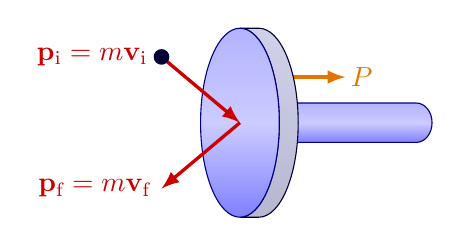
\begin{tikzpicture}
  \def\Ra{0.5}
  \def\Rb{1.2}
  \def\ra{0.20}
  \def\rb{0.25}
  \def\w{0.12}  % wall thickness
  \def\l{2}     % piston length
  \def\ang{140} % momentum angle
  \def\p{1.3}   % momentum length
  
  % PISTON
  \draw[->,very thick,orange!90!black] (2*\w,{0.4*(\rb+\Rb)}) --++ (0.55*\l,0)
    node[right=-2,orange!90!black] {$P$};
  \draw[piston]
    (2*\w,\rb) --++ (\l,0) arc (90:-90:{\ra} and {\rb}) --++ (-\l,0) -- cycle;
  \draw[walldark]
    (0,\Rb) arc (90:-90:{\Ra} and {\Rb}) --++ (2*\w,0) arc (-90:90:{\Ra} and {\Rb}) -- cycle;
  \draw[piston] (0,0) ellipse ({\Ra} and \Rb);
  
  % GAS PARTICLE
  \draw[->,very thick,red!80!black]
    (\ang:\p) node[left=1] {$\vb{p}_\text{i} = m\vb{v}_\text{i}$} coordinate (I) -- (0,0);
  \draw[->,very thick,red!80!black]
    (0,0) -- (-\ang:\p) node[left] {$\vb{p}_\text{f} = m\vb{v}_\text{f}$};
  \node[circle,fill,inner sep=2,fill=black!80!blue] at (I) {};
  
\end{tikzpicture}



\end{document}
